\chapter{Implementierung} \label{sec:implementation}

Dieses Kapitel widmet sich der Umsetzung der in Kapitel \ref{sec:optimization} beschriebenen Verfahren. Hierfür wurden im Laufe dieser Arbeit verschiedene Prototypen entwickelt, die jeweils als Proof of Concept für die einzelnen Verfahren galten. Ziel dieser Umsetzung ist es einen einzigen Prototypen in Form einer App auf dem Project Tango Gerät zu entwickeln, die den gesamten Funktionsumfang, welcher in Kapitel \ref{sec:final_prototype} zusammengefasst wird, beinhaltet. \\

Zudem muss ein Programmfluss geschaffen werden, der es ermöglicht, in die Daten des Tiefenbuffers mit eigenen Implementierungen eingreifen zu können, um ein Filtern zu ermöglichen. Wie das technisch ermöglicht wird, und auf welcher Basis die Anwendung implementiert wird, beschreibt das Kapitel \ref{eq:technic}. Hiernach werden die Umsetzung der die jeweiligen Verfahren näher erläutert.

\section{Finaler Prototyp} \label{sec:final_prototype}

Der finale Prototyp soll, wie bereits erwähnt, alle zuvor beschriebenen Verfahren zur Realisierung von Überlagerungen in einer Augmented Reality Szene beinhalten. Also muss zunächst eine einfache AR Szene geschaffen werden, in der eine virtuelle Kamera existiert, die die intrinsischen und extrinsischen Eigenschaften der Project Tango Kamera zu jeder Zeit entspricht. Außerdem muss das aktuelle Farbbild der RGB Kamera in der Szene im Hintergrund dargestellt werden. Für diese Aufgaben existieren, wie bereits in Kapitel \ref{sec:theory_project_tango} erwähnt, Schnittstellen, die diese Informationen liefern. \\

Um eine reale Überdeckung sinnvoll testen zu können, benötigen wir zudem ein virtuelles Objekt in der Szene. Dieses sollte im Idealfall nicht zu einfach gestaltet sein, damit die Verfahren anhand realistischen Gegebenheiten verglichen werden können. Zu diesem Zweck sollen Objekte in die App eingelesen werden können, die in in dem Forschungsbereich der Computergraphik typischerweise eingesetzt werden. Typische Modelle sind zum Beispiel der \enquote{Utah Teapot}, \enquote{Stanford Bunny} oder \enquote{Blenders Suzanne}\footnote{List of common 3D test models - https://goo.gl/MsOtSW}.  Eines dieser Modelle soll in die Szene geladen werden und es soll die Möglichkeit gegeben sein, dass das Objekt flexibel positioniert werden kann. Hierzu wird zudem der beschriebene Raypicking Mechanismus umgesetzt.\\

Um die Ergebnisse der  realen Überlagerung einfach gegenüberstellen zu können, sollen die beschriebenen Tiefenbild generierenden Verfahren flexibel im Betrieb ausgetauscht werden. Dazu gehört das Rendering der Pointcloud Projektion, die TSDF Rekonstruktion durch Chisel und die Ebenen Rekonstruktion. Außerdem soll das Filtern des Tiefenbildes mit Hilfe des Guided Filter optional zu jeder Zeit möglich sein. Hilfreich wäre es zudem, die Einstellungen des Guided Filters flexibel einstellen zu können. Wie diese Verfahren und ihre Flexibilität umgesetzt wird in den folgenden Kapiteln näher beschrieben.

\section{Technische Umsetzung und Struktur} \label{eq:technic}

Wie bereits erwähnt, basiert das Project Tango System auf Googles Android Betriebsystem. Dies ermöglicht es Anwendungen mit bestehenden und bewerten Technologien wie OpenGL, Rajawali\footnote{Android OpenGL ES 2.0/3.0 Java Engine - https://goo.gl/r9Ohdj (27.02.16)} oder der Unity Engine entwickeln zu können. Project Tango bietet hierfür drei verschiedene Schnittstellen, in C/C++, Java und Unity (Mono Framework in C\#), um auf die Sensordaten in verschiedenen Umgebungen zugreifen zu können. Im laufe dieser Arbeit wurden alle Schnittstellen mit verschiedensten prototypischen Entwicklungen getestet.\\

Der finale Prototyp wurde letztendlich in C/C++ entwickelt und basiert auf dem Android NDK\footnote{Android Native Development Kit - http://goo.gl/ananZT (27.02.16)}. Letztendlich greifen die anderen, höher angesiedelten Schnittstellen auf genau die selbe native Implementierung zurück, um sie in Java und Unity zu Verfügung zu stellen. Außerdem ermöglicht die native Entwicklung, neben Performancevorteilen, den vollen Zugriff auf OpenGL Mechanismen, die von Rajawali gegebenenfalls ausgeschlossen werden. \\

Das Projekt Tango Team stellt für die native Entwicklung die eigentliche Tango Schnittstellen Bibliothek\footnote{Project Tango C API - https://goo.gl/lbBfAp (27.02.16)}, eine Support-Bibliothek\footnote{Project Tango C Suppport API - https://goo.gl/VGyeKm (27.02.16)} und eine einfache Kapselung für OpenGL Anwendungen mit dem Namen TangoGL\footnote{TangoGL Repository - https://goo.gl/ymDCsJ (27.02.16)} an. Die Support-Bibliothek bietet verschiedene Hilfsfunktionen zur Datenverarbeitung und Allokation. TangoGL wiederum erleichtert den Einstieg in die OpenGL Entwicklung und übernimmt die Grundlegende Struktur und Interoperabilität zu Project Tango. Zum Beispiel gibt es Methoden, um Tango Positionsdaten in eine Translationsmatrix umrechnen zu können oder Klassen, die das Rendern der aktuellen RGB Kamera Textur übernehmen. \\

Abbildung \ref{fig:structure} zeigt grob den strukturellen Aufbau der Android Applikation. Der obere Teil der Grafik bezieht sich dabei auf den in Java implementierten Teil, der die Nutzeroberfläche, ihre Interaktion und den Renderingcanvas beinhaltet. Die Activity stellt jedoch nur einen kleinen Teil der Anwendung dar, denn alle Interaktionen und Ereignisse werden über ein Java Native Interface (JNI) zum nativen Teil der Anwendung geleitet, welcher die Ansprache der Schnittstellen, die Prozesslogik und das Rendering selbst beinhaltet. \\

\begin{figure}[h]
  \centering
	\includegraphics[width=1.0\textwidth]{content/images/implementation/uml.png} 
  \caption{Struktureller Aufbau des Prototypen}
  \label{fig:structure}
\end{figure}

Die Hauptklasse \enquote{ARApp} in der Grafik widmet sich in der Anwendung nur der Anreicherung und Weiterleitung von JNI Informationen und der Ansprache der Project Tango Schnittstelle. Kern der Anwendung ist die \enquote{Scene} Klasse, welche die Informationen an das entsprechend aktive Verfahren zur Tiefenbild Generierung weiterreicht. So wird zum Beispiel die Pointcloud an das Chisel, Pointcloud oder Plane Drawable weitergereicht, damit Sie ein aktualisiertes Tiefenbild rendern können. Auch das Farbbild der Kamera gelangt über die Scene zum RGB Drawable. Die Szene selbst ermöglicht durch den Einsatz von OpenCV\footnote{Open Source Computer Vision - http://opencv.org/} den optionalen Filter Prozess durch den Guided FIlter. Um das zu ermöglichen wird ein OpenGL Framebuffer eingesetzt. Das Listing \ref{lst:rendering} zeigt das Vorgehen beim Rendering der Szene.\\

\begin{lstlisting}[mathescape,caption=Rendering der Szene, label=lst:rendering]
Eingang: Farbbild $rgb$, Zusatz Tiefenbuffer $tb$
         Haupt Frambuffer $fb$ mit Farb und Tiefenanteil
Ausgang: Resultierendes Hauptbild $fb$

Leere $fb$ und $tb$

Wenn die Pointcloud Projektion aktiv ist
    Rendere die Tiefe der Pointcloud auf $tb$
Wenn die Chisel Rekonstruktion aktiv ist
    Rendere die Tiefe der Chisel Rekonstruktion  auf $tb$
Wenn die Ebenen Rekonstruktion aktiv ist
    Rendere die Tiefe der Ebenen Rekonstruktion auf $tb$
    
Wenn gefiltert werden soll
    Wende den GuidedFilter auf $tb$ mit $rgb$ als Guide an
        
Rendere $rgb$ auf $fb$ 
ersetzte den Tiefenbuffer von $fb$ druch $tb$
aktiviere den OpenGL Depth Test
rendere das 3D Modell auf $fb$
\end{lstlisting}

\section{Umsetzung der Verfahren}

\subsubsection*{Tiefe aus der Pointcloud Projektion}

Wie im Kapitel \ref{sec:pc-projection} erwähnt müssen die Punkte der Project Tango Pointcloud auf die Bildebene projiziert werden und mit einer entsprechenden Tiefenfarbe und einem Radius auf den Tiefenpuffer gezeichnet werden. Dieser Schritt wurde auch bereits in Prototoypen mit den angegebenen Gleichungen umgesetzt. Jedoch kann man sich hierfür das OpenGL Rendering zu Nutze machen und die Projektion OpenGL übernehmen lassen. Denn OpenGL unterstützt für das Rendering neben Polygonen auch primitiven wie Punkte und Linien.  Zudem lässt sich durch einen entsprechenden Fragmentshader die Größe der Punkte entsprechend anpassen.




\subsubsection*{Planare Rekonstruction}

Der erste Proof of Concept Prototyp wurde zu Beginn dieser Arbeit auf Java Ebene implementiert und entwickelte sich nach und nach zu dem in \ref{sec:plane-reconstruction} beschriebenen Verfahren. Für die finale Umsetzung in dem nativen Prototypen mussten somit alle Algorithmen und Datenstrukturen neu in C/C++ umgesetzt werden. Begonnen wurde mit dem Octree, der in seinen tiefsten Zweigen die Menge aller aufgenommenen Punkte für den jeweiligen Sektor und eine Instanz der \enquote{Reconstructor} Klasse beinhaltet. Diese beinhaltet alle beschriebenen Algorithmen zur Ebenenrekonstruktion wie RANSAC, dem Graham Scan und der linearen Regression. \\

\begin{figure}[h]
  \centering
	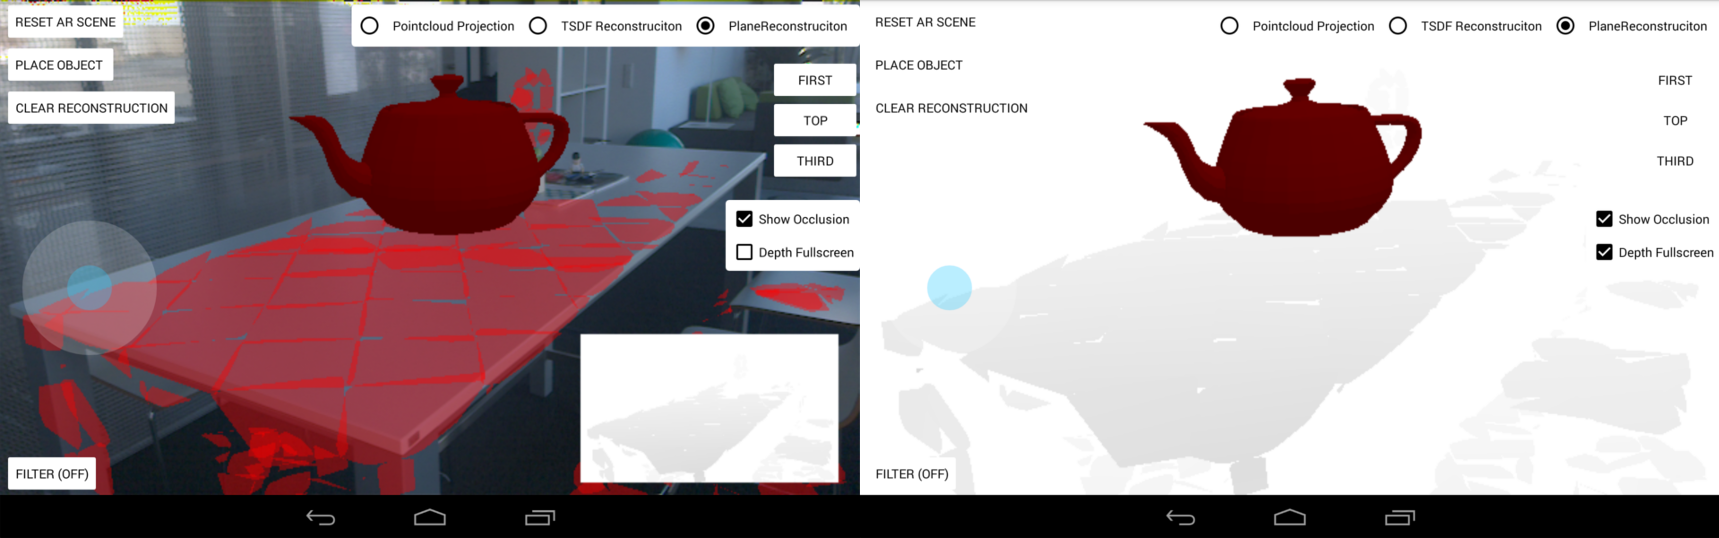
\includegraphics[width=1.0\textwidth]{content/images/implementation/plane-demo.png} 
  \caption{Planare Rekonstruktion Prototyp. Links optionale Projektion auf der Bildebene. Rechts das resultierende Tiefenbild.}
  \label{fig:plane-demo}
\end{figure}

Für die Berechnung mit Vektoren und Matrizen wurde wie auch im gesamten Projekt die OpenGL Mathematics Bibliothek (GLM)\footnote{OpenGL Mathematics - http://goo.gl/2oY83s (27.02.16)} verwendet. Sie bietet typische Primitiven mit entsprechenden Operationen für Berechnungen der linearen Algebra. Wie bereits beschrieben wird für die lineare Regression die Berechnung von Eigenvektoren mit ihren Eigenwerten benötigt. Diese Berechnung wird von GLM nicht unterstützt. Hier wurde die Eigen-Bibliothek\footnote{Eigen: template library for linear algebra - http://goo.gl/TsNOuW (27.02.16)} verwendet, die diese Operation für den Anwender anbietet. Abbildung \ref{fig:plane-demo} zeigt die Ergebnisse der Ebene Rekonstruktion Links und der daraus Resultierenden Tiefeninformation Rechts.




\subsubsection*{TSDF Rekonstruktion}

\citet{Klingensmith_2015_7924} erwähnen, dass ihr Verfahren Chisel zunächst als proprietäre Umsetzung im Project Tango Constructor\footnote{Project Tango Constructor - https://goo.gl/8HdTnY (27.02.16)}, Googles Demo Anwendung zur räumlichen Rekonstruktion, umgesetzt wurde. Zu Ihrer Publikation haben sie jedoch zusätzlich eine Open-Source ROS basiertes Modul zur Verfügung gestellt. Diese Bibliothek mit dem Namen OpenChisel\footnote{OpenChisel - Chisel chunked TSDF library - https://goo.gl/nla8hy (27.02.16)} wurde für den Prototypen auf Android NDK portiert. Dafür wurden einige Module des C++11 Standards, wie zum Beispiel \enquote{st::shared\_ptr}, die zum derzeitigen Kenntnisstand vom Android NDK nicht unterstützt werden, auf die Boost\footnote{Boost C++ Libraray - http://www.boost.org/ (27.02.16)} Implementationen abgeändert. Neben der Boost Bibliothek nutzt OpenChisel auch die Eigen Bibliothek für Primitiven und Berechnungen der linearen Algebra.\\

Als Eingabe benötigt OpenChisel neben der Kameraposition und Kameraeigenschaften entweder einer Pointcloud oder ein Tiefenbild. In der Proof of Concept Umsetzung war erkennbar, dass OpenChisel mit der Pointcloud von Project Tango deutlich schlechtere Ergebnisse lieferte, als die Implementation des Constructors von Google. Dadurch die Support Bibliothek von Google seit Februar 2016 eine performante Methode\footnote{TangoSupport\_upsampleImageNearestNeighbor - https://goo.gl/mchIie (27.02.16)} anbietet, um aus einer Punktewolke eine DepthMap mit einer Auflösung von \(320x180 \) zu generieren, wird nun ein Tiefenbild für OpenChisel verwendet. Die resultierenden Ergebnisse kommen dadurch der Constructor Implementation deutlich näher. Abbildung \ref{fig:chisel-demo} zeigt eine exemplarische Rekonstruktion eines Tiefenbildes links mit dem resultierenden Tiefenbild rechts.

\begin{figure}[h]
  \centering
	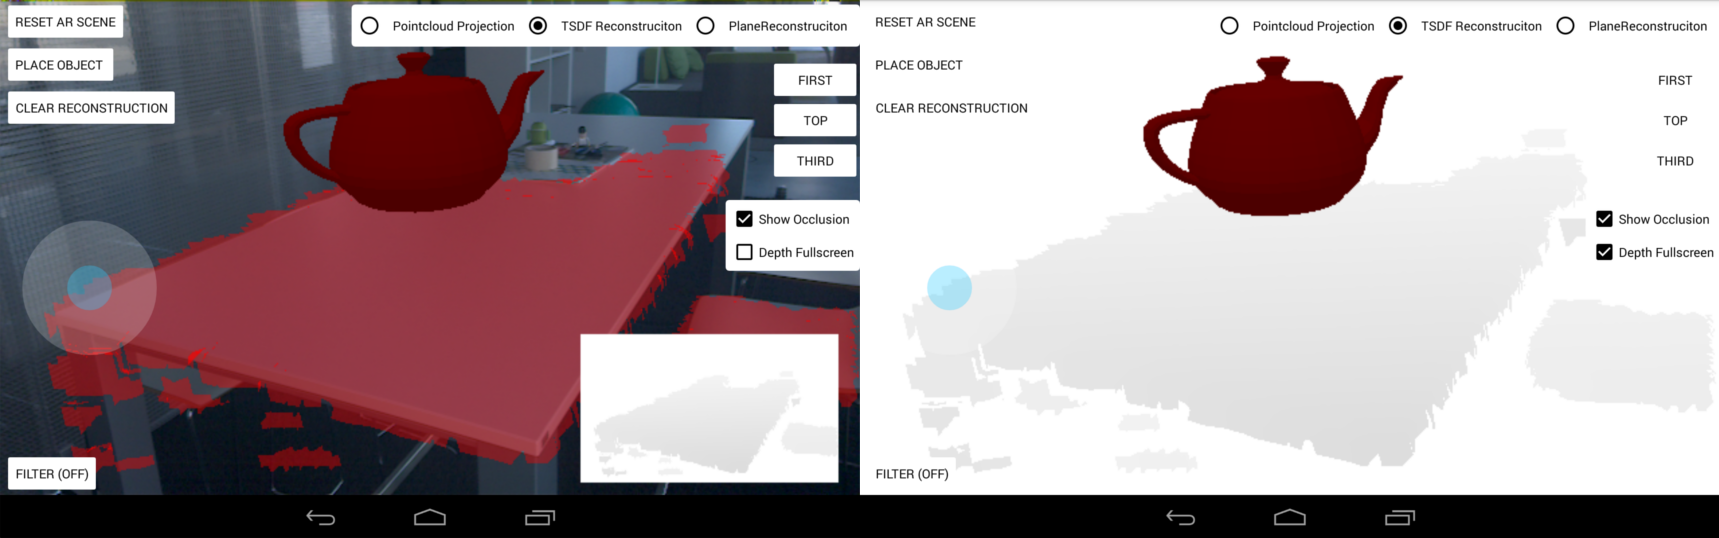
\includegraphics[width=1.0\textwidth]{content/images/implementation/chisel-demo.png} 
  \caption{OpenChisel Rekonstruktion Prototyp. Links optionale Projektion auf der Bildebene. Rechts das resultierende Tiefenbild.}
  \label{fig:chisel-demo}
\end{figure}


\subsubsection*{Guided Filter}

Für die Anwendung des Guided Filters wurde, wie bereits erwähnt, die Computer Vision Bibliothek OpenCV verwendet. Um diesen Filter mit OpenCV anwenden zu können mussten zuvor das RGB Bild und das Tiefenbild in das OpenCV Format gebracht werden. Dies war jedoch mit den Methoden \enquote{glReadPixels} und \enquote{glTexImage2D} für den aktuell selektierten Framebuffer und der OpenGL Textur problemlos möglich. Zwar sind die Speicherkonventionen von OpenGL und OpenCV, was die X und Y Achse angeht, genau vertauscht, jedoch ist das Filtern, welches daraus folgend gedreht stattfindet, für den Nutzer völlig intransparent und muss nicht weiter berücksichtigt werden.\\

Problematisch ist jedoch, dass das OpenGL Tiefenbild eine Farbtiefe von 16Bit nutzt und der OpenCV Guided Filter nur auf 8Bit Graustufen angewendet werden kann. Diese Transformation und die daraus resultierende Ungenauigkeit der Tiefe wurde jedoch zunächst in Kauf genommen, da erst einmal der Mechanismus als solches getestet werden soll. In der späteren Auswertung von Testszenarien muss diese Transformation berücksichtigt werden. \\

Diese Implementierung ermöglicht es, den Guided Filter dynamisch auf das aktuell generierte Tiefenbild mit dem aktuell aufgenommen RGB Bild als Leitbild anzuwenden. Außerdem lassen sich die Filter Parameter, dem Radius \(r\) und den Einflussfaktor \(\epsilon\) dynamisch variieren. Abbildung \ref{fig:filter-demo} zeigt das Tiefenbild der TSDF Rekonstruktion links, auf die rechts der Guided Filter mit dem aktuellen RGB Bild angewendet wurde. \\

\begin{figure}[h]
  \centering
	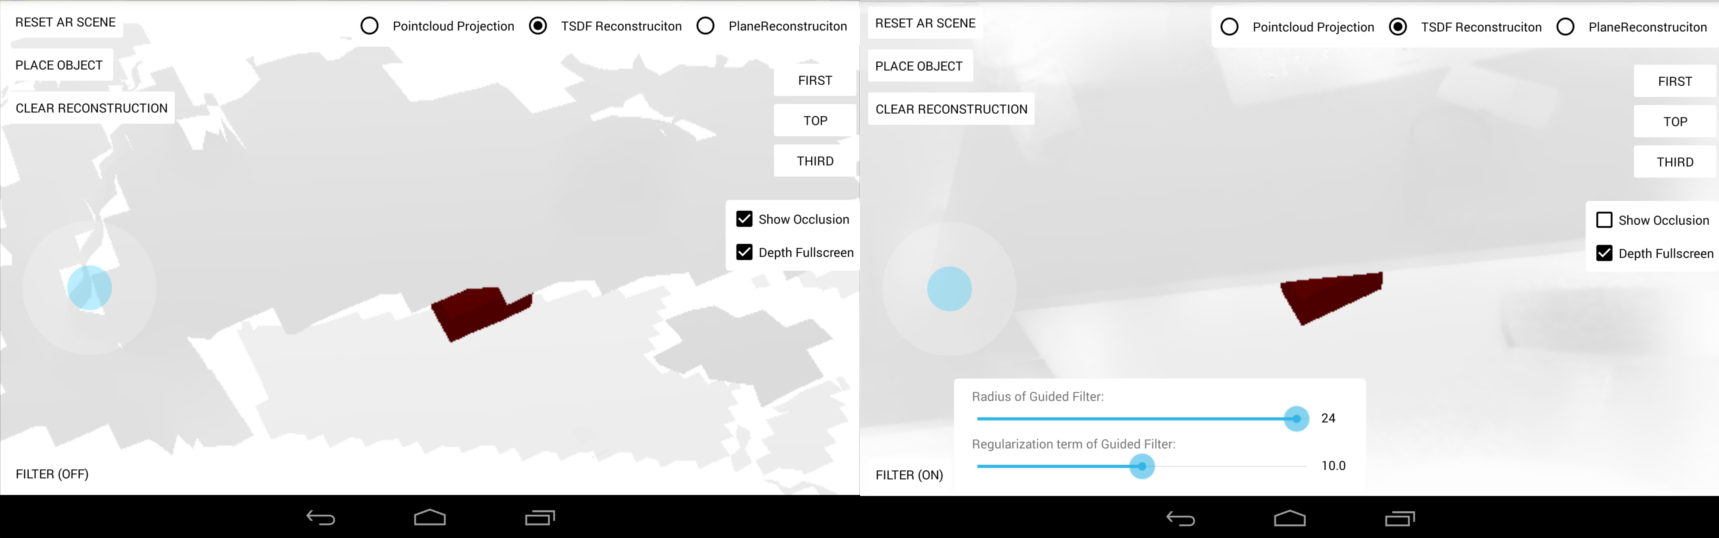
\includegraphics[width=1.0\textwidth]{content/images/implementation/filter-demo.png} 
  \caption{Anwendung des Guided Filters auf eine TSDF Rekonstruktion. Links vor und rechts nach der Anwendung.}
  \label{fig:filter-demo}
\end{figure}


\section{Technische Problemstellungen}

Auch wenn schon einige Probleme in der Umsetzung der jeweiligen Verfahren in Kapitel \ref{sec:method-implementation} näher beschrieben wurden, werden hier noch Einzelheiten aufgegriffen, die bei der Entwicklung für Projekt Tango zu beachten waren. \\

Alle von Project Tango zurückgegeben Vektoren besitzen Ihre eigene Konvention bezüglich der Achsenanordnungen. Gegenüber der Konvention in OpenGL sind die Achsen \(Z\) und \(Y\) vertauscht. Außerdem zeigt die resultierende \(Z\)-Achse in die gegengesetzte Richtung. Aufgrund dieser Unterschiedlichen Konvention müssen alle Vektoren \(\vec{v}\) von Project Tango mit der Transformationsmatrix \(T_{OGL}^{PT}\) aus Gleichung \ref{eq:transformation} konvertiert werden \citep{Proje15:online}. Nachdem Google im Laufe dieser Arbeit neue Schnittstellen\footnote{Project Tango API: Transformation Support - https://goo.gl/N8dapq (29.02.16)} zur Verfügung gestellt haben, um diese Transformationen zu abstrahieren, können die \enquote{TransformationSupport} Methoden hierfür genutzt werden.

\begin{equation} \label{eq:transformation}
T_{OGL}^{PT} =\left( \begin{matrix} 1&0&0&0\\0&0&-1&0\\0&1&0&0\\0&0&0&1 \end{matrix} \right)
\end{equation}

\textbf{TODO:} ggf mit anderem Kapitel zusammenführen wenn nicht mehr zusammenkommt


